\chapter{Appendix}

\section{Daily Schedule}

\begin{minipage}{.5\textwidth}
  \begin{center}
  Monday, Tuesday, Thursday, Friday\\
  \begin{tabular}{|r|l|}
    \hline
    8:00-8:50		&Block   \\
    \hline    
    8:55-9:45		&Block   \\
        \hline
    9:50-1020	&	Flex   \\
    \hline    
    10:25-11:15	&Block   \\
    \hline    
    11:15-12:40	&M       \\
      \hline  
    12:40-1:30	&	Block  \\
      \hline  
    1:35-2:25		&Block   \\
      \hline  
    2:30-3:20		&Block   \\
        \hline
    3:20-4:00		&X\\
        \hline
  \end{tabular}\end{center}
\end{minipage}
\begin{minipage}{.5\textwidth}
\begin{center}Wednesday\\
\begin{tabular}{|r|l|}
      \hline
8:00-8:45		&Faculty   \\
    \hline
8:55-9:45		&Block     \\
    \hline
9:50-10:40	&	Block    \\
    \hline
10:40-10:50	&	Break    \\
    \hline    
10:50-11:40	&Block     \\
    \hline
11:40-12:40	&M         \\
    \hline
12:40-1:30	&	Block    \\
    \hline
1:35-2:25		&Block     \\
    \hline
2:30-3:20		&Block     \\
    \hline
3:20-4:00		&X\\
    \hline
\end{tabular}  \end{center}
\end{minipage}

\section{Activity Schedules}


\begin{minipage}{.5\textwidth}
  \begin{center}
45 Minute Activity Period\\
\begin{tabular}{|r|l|}
    \hline
  8:00-8:50 &Block     \\
    \hline
  8:55-9:45 &Block     \\
    \hline
  9:50-10:35 &Activity \\
    \hline
  10:40-11:30 &Block   \\
    \hline
  11:30-12:40 &M       \\
    \hline
  12:40-1:30 &Block    \\
    \hline
  1:35-2:25 &Block     \\
    \hline
  2:30-3:20 &Block     \\
    \hline
  3:20-4:00 &X         \\
    \hline
\end{tabular}
\end{center}
\end{minipage}
\begin{minipage}{.5\textwidth}
  \begin{center}
60 Minute Activity Period\\
\begin{tabular}{|r|l|}
  \hline
 8:00-8:50 &Block     \\
  \hline
 8:55-9:45 &Block     \\
   \hline
 9:50-10:05 & Break   \\
   \hline
 10:10-11:00 &Block   \\
   \hline
 11:00-12:15 &M       \\
   \hline
 12:15-1:05  &Block   \\
   \hline
 1:10-2:00  &Block    \\
   \hline
 2:05-2:55  &Block    \\
   \hline
 3:00-4:00 &Activity \\ 
   \hline
\end{tabular}
 \end{center}
\end{minipage}
















\newpage
\section{Forms}

The following forms will allow you to request an academic overload, departmental overload, Independent Study, or MSON class.  You may hand-write or type your responses to the forms.  Submit your completed request(s) via email to the Assistant Head of School for Academic Affairs\footnote{\href{mailto:jonathan.gray@indiansprings.org}{Dr. Gray}} with clear subject lines, e.g. 

\begin{itemize}
  \item Academic Overload Request - Student Name
  \item Departmental Overload Request - Student Name  
  \item Independent Study Request - Student Name
  \item MSON Course Request - Student Name
\end{itemize}

\newpage

\subsection{Academic Overload Form}

An academic overload is defined as enrolling in seven or more classes in a semester. Note that your performance will be reviewed at the initial quarter of the overloaded term and periodically throughout the academic year.  Students who are struggling may be required to remove any overloads at that time.  

\vspace{.5cm}


\begin{tabular}{ll}
Student Name: & \underline{\hspace{7cm}}\\
&\\
Grade Level:  & \underline{\hspace{7cm}}\\
&\\
Expected Courses: & \underline{\hspace{7cm}}\\
&\\
& \underline{\hspace{7cm}}\\
&\\
& \underline{\hspace{7cm}}\\
&\\
& \underline{\hspace{7cm}}\\
&\\
& \underline{\hspace{7cm}}\\
&\\
& \underline{\hspace{7cm}}\\
&\\
& \underline{\hspace{7cm}}
\end{tabular}



 
 
 
 
 
 
 
\begin{enumerate}
  \item Provide all extracurricular commitments at Springs.
  
  \vfill
  
  \item Provide all regular commitments you have outside of Springs (music lessons, athletic clubs, etc.) and how much time per week they require.
  
  \vfill
  
  \item Articulate your rationale for your requested overload(s).
  
  \vfill
  
\end{enumerate} 






































\newpage

\subsection{Departmental Overload Form}

A departmental overload is defined as taking two or more courses in a department during an academic term.  Note that your performance will be reviewed at the initial quarter of the overloaded term and periodically throughout the academic year.  Students who are struggling may be required to remove any overloads at that time.  \\

Please list all previous courses in the given department, during which grade you took them, and your final course grade (or most recent grade).








\renewcommand{\arraystretch}{2}
\begin{tabular}{lccc}
  & \hspace{2cm} Previous Course  \hspace{2cm} & Grade Level & Grade \\
  1.& \underline{\hspace{7cm}} &\underline{\hspace{1cm}} &\underline{\hspace{1cm}} \\
  2.& \underline{\hspace{7cm}} &\underline{\hspace{1cm}} &\underline{\hspace{1cm}} \\
  3.& \underline{\hspace{7cm}} &\underline{\hspace{1cm}} &\underline{\hspace{1cm}} \\
  4.& \underline{\hspace{7cm}} &\underline{\hspace{1cm}} &\underline{\hspace{1cm}} \\
  5.& \underline{\hspace{7cm}} &\underline{\hspace{1cm}} &\underline{\hspace{1cm}} \\
  6.& \underline{\hspace{7cm}} &\underline{\hspace{1cm}} &\underline{\hspace{1cm}} 
\end{tabular}

\vspace{1cm}
\noindent\hrulefill
\vspace{.5cm}

\renewcommand{\arraystretch}{1}
\noindent\begin{tabular}{ll}
Parent/Guardian Signature: & \underline{\hspace{7cm}}\\
&\\
Advisor Signature:  & \underline{\hspace{7cm}}\\
&\\
Department Chair Signature: &  \underline{\hspace{7cm}}\\
&\\
Academic Committee’s Decision:	& Approved  \hspace{.5cm} 	Not Approved
\end{tabular}\\

\vspace{.5cm}
 


\vspace{1cm}



%\noindent \underline{Department Chairs}
%\bmc{2}
%\begin{enumerate}\itemsep=0mm
%\item[] Art:  Clay Colvin
%\item[] Computer Science:  William Belser
%\item[] English:  James Griffin
%\item[] History:  Kelly Jacobs
%\item[] Languages:  William Blackerby
%\item[] Math:  Stephanie Thomas
%\item[] Physical Education:  Greg Van Horn
%\item[] Science:  Tessa Magnuson
%\end{enumerate}\etc


\newpage

\subsection{AP Exam Request Form}

\vspace{1cm}

\begin{tabular}{ll}
Student Name: & \underline{\hspace{7cm}}\\
&\\
Grade Level:  & \underline{\hspace{7cm}}\\
&\\
Date Requested: &  \underline{\hspace{7cm}}\\
&\\
AP Exam Request(s): & \underline{\hspace{7cm}}\\
&\\
& \underline{\hspace{7cm}}\\
&\\
& \underline{\hspace{7cm}}\\
&\\
& \underline{\hspace{7cm}}\\
&\\
& \underline{\hspace{7cm}}
\end{tabular}

\vspace{1cm}

\noindent Explain how you will prepare for these additional AP exam(s).\footnote{A class, online course, tutor, independent study; course study guide, etc.}








\vspace{4cm}
\noindent List all AP exam(s) you will take as part of an enrolled AP course at Springs:

\vspace{.25cm}
\begin{enumerate}
  \item \underline{\hspace{9cm}}
  \item \underline{\hspace{9cm}}
    \item \underline{\hspace{9cm}}
  \item \underline{\hspace{9cm}}
  \item \underline{\hspace{9cm}}
  \item \underline{\hspace{9cm}}
  \item \underline{\hspace{9cm}}            
\end{enumerate}






















\newpage


\subsection{Independent Study Form}

\vspace{1cm}



\begin{tabular}{ll}
Student Name: & \underline{\hspace{7cm}}\\
&\\
Course Name:  & \underline{\hspace{7cm}}\\
&\\
Faculty Advisor(s):&  \underline{\hspace{7cm}}\\
&\\
Term: & Fall Only\\
&\\
& Spring Only\\
&\\
& Fall and Spring
\end{tabular}\\












Please type your answers to the following question on a separate sheet of paper and include with this form. 

\begin{enumerate}


  \item What are the goals of your proposed course?
  \item What are the essential questions you wish to answer in your studies?
  \item What texts and/or resources will you need to engage in the course?
  \item How will you be assessed for learning and mastery? (Include quantity, length, and frequency.) 
  \item What is your proposed meeting schedule with your advisor? (Be specific.) 
  \end{enumerate}

\noindent Upon completing the steps above, please read and sign the following: \\

I agree to faithfully meet all obligations, including scheduled meeting times, assessments, and methods of study, identified above. Failure to do so will result in not receiving credit for the Independent Study. \\

\renewcommand{\arraystretch}{1}
\noindent\begin{tabular}{ll}
Student Signature:  & \underline{\hspace{7cm}}\\

\end{tabular}\\


\vspace{.5cm}

\vfill

\noindent \hrulefill For Internal Use \hrulefill 

\vspace{.5cm}

\noindent I agree to sponsor the Independent Study described herein.\\

\renewcommand{\arraystretch}{1}
\noindent\begin{tabular}{ll}
Advisor Signature:  & \underline{\hspace{7cm}}\\
&\\
Academic Committee’s Decision:	& Approved  \hspace{.5cm} 	Not Approved
\end{tabular}\\





\newpage
\subsection{MSON Enrollment Form}

\noindent \textbf{Malone School Online Networks Course Policies}


Note that MSON online courses meet at a fixed time, typically twice per week.  Because they do not fit into our rotating schedule, students will regularly miss their scheduled classes while attending their MSON course. 

\begin{enumerate}\itemsep=0mm
\item You must be a junior or senior to enroll.
\item The average from your core courses (English, History, Science, Math, Languages) from the “Quarter 3 - Report” must be at least 90.
\item You must have a good attendance record. 
\item The MSON course cannot be taken in place of an identical, or almost identical, course offered by the school, assuming the school course can be made to fit into your schedule. 
\item The course must be your 6th class (not counting PE in 11th grade). 
\item The course must be taken for credit. 
\item You must comply with the advertised add/drop dates, course prerequisites and the attendance and homework policies of the MSON instructor. 
\item You are responsible for catching up work that you miss from a Springs course because of your attendance at an MSON course.  \emph{This includes notifying your teacher at Springs ahead of every missed class.}  
\item Per MSON policy, their courses must be prioritized over all other courses/obligations.  This means you may have classes during a school break/holidays, other classes, choir, sports, and so on.  
\end{enumerate}



By signing this document, I agree to the policies as stated above.

\vspace{.75cm}

\hfill Student Signature: \underline{\hspace{3in}}

\vspace{.5cm}

\noindent\hrulefill

\vspace{.5cm}

\hfill Student Name: \underline{\hspace{3in}}

\vspace{1cm}

\hfill Current Grade Level:  \underline{\hspace{3in}}

\vspace{1cm}

\hfill Average from Core Courses in Q$3$R:\underline{\hspace{3in}}

\vspace{1cm}

\hfill Requested MSON Course(s):\underline{\hspace{3in}}

\vspace{1cm}

\hfill Endorsing Teacher (Signature):\underline{\hspace{3in}}



\newpage
\section{Sample Academic Paths}

  
\bmc{2}

  \begin{tabular}{l}
\vspace{.01mm}\textbf{{Grade 9}}\\
\indent {\footnotesize English 9 }\\
\indent {\footnotesize Spanish I }\\
\indent {\footnotesize World History: To 1500 }\\
\indent {\footnotesize Algebra I }\\
\indent {\footnotesize Biology }\\
\indent {\footnotesize Intro to Engineering - 3D Design }\\
\indent {\footnotesize WellFit  }\\
\indent {\footnotesize 9th Grade PE  }\\
\end{tabular}

\vspace{1cm}

\begin{tabular}{l}
    \vspace{.01mm}\textbf{{Grade 10}}\\
\indent {\footnotesize Critical Reading \& Analytical Writing } \\
\indent {\footnotesize Spanish II }\\
\indent {\footnotesize AP European History }\\
\indent {\footnotesize Geometry } \\
\indent {\footnotesize Chemistry } \\
\indent {\footnotesize Art History } \\
\indent {\footnotesize 10th Grade PE } \\
\end{tabular}

\vspace{1cm}

\begin{tabular}{l}
    \vspace{.01mm}\textbf{{Grade 11}}:\\ 
\indent {\footnotesize Literary Analysis } \\
\indent {\footnotesize The Art of the Personal Narrative }\\
\indent {\footnotesize Spanish III }\\
\indent {\footnotesize AP United States History }\\
\indent {\footnotesize Economics }\\
\indent {\footnotesize Algebra II w/ Trigonometry }\\
\indent {\footnotesize Conceptual Physics }\\
\indent {\footnotesize 11th Grade PE }\\
\indent {\footnotesize Injury Prevention \& Weight Training }\\
\end{tabular}

\vspace{1cm}

\begin{tabular}{l}
\vspace{.01mm}\textbf{{Grade 12}}\\
\indent {\footnotesize Shakespearean Comedies \& Tragedies }\\
\indent {\footnotesize The Graphic Novel }\\
\indent {\footnotesize American Government }\\
\indent {\footnotesize Religious Literacy }\\
\indent {\footnotesize Precalculus }\\
\indent {\footnotesize AP Environmental Science }\\
\indent {\footnotesize Digital Photography }\\
\indent {\footnotesize Foundation of Sports Medicine \& Safety }\\
 \end{tabular}\columnbreak
 
  \begin{tabular}{l}
\vspace{.01mm}\textbf{{Grade 9}}\\
\indent {\footnotesize English 9 }\\
\indent {\footnotesize Spanish IV }\\
\indent {\footnotesize World History: To 1500 }\\
\indent {\footnotesize Adv Algebra II }\\
\indent {\footnotesize Biology }\\
\indent {\footnotesize Stagecraft }\\
\indent {\footnotesize WellFit  }\\
\indent {\footnotesize 9th Grade PE  }\\
\end{tabular}

\vspace{1cm}

\begin{tabular}{l}
    \vspace{.01mm}\textbf{{Grade 10}}\\
\indent {\footnotesize Critical Reading \& Analytical Writing } \\
\indent {\footnotesize AP Spanish Language }\\
\indent {\footnotesize AP European History }\\
\indent {\footnotesize Adv Precalculus } \\
\indent {\footnotesize Chemistry } \\
\indent {\footnotesize Music History } \\
\indent {\footnotesize Intro Music Theory } \\
\indent {\footnotesize AP Music Theory } \\
\indent {\footnotesize 10th Grade PE } \\
\end{tabular}

\vspace{1cm}

\begin{tabular}{l}
    \vspace{.01mm}\textbf{{Grade 11}}:\\ 
\indent {\footnotesize Literary Analysis } \\
\indent {\footnotesize Film Rhetoric }\\
\indent {\footnotesize AP United States History }\\
\indent {\footnotesize Economics }\\
\indent {\footnotesize Calculus }\\
\indent {\footnotesize AP Biology }\\
\indent {\footnotesize AP Environmental Science }\\
\indent {\footnotesize Adv Contemporary Music Ensemble } \\
\indent {\footnotesize Adv Performance Ensemble } \\
\indent {\footnotesize 11th Grade PE }\\
\end{tabular}

\vspace{1cm}

\begin{tabular}{l}
\vspace{.01mm}\textbf{{Grade 12}}\\
\indent {\footnotesize Art of the Personal Narrative }\\
\indent {\footnotesize Creative Writing Workshop }\\
\indent {\footnotesize AP Statistics }\\
\indent {\footnotesize Conceptual Physics }\\
\indent {\footnotesize Adv Acting } \\
\indent {\footnotesize Adv Contemporary Music Ensemble } \\
\indent {\footnotesize Choral Conducting \& Literature }\\
\indent {\footnotesize Directing \& Stage Management }\\
 \end{tabular}



\etc
%\section{FAQ}

\newpage
\thispagestyle{empty}

\mbox{ }
\vspace{-2cm}
\hspace{-2.5cm}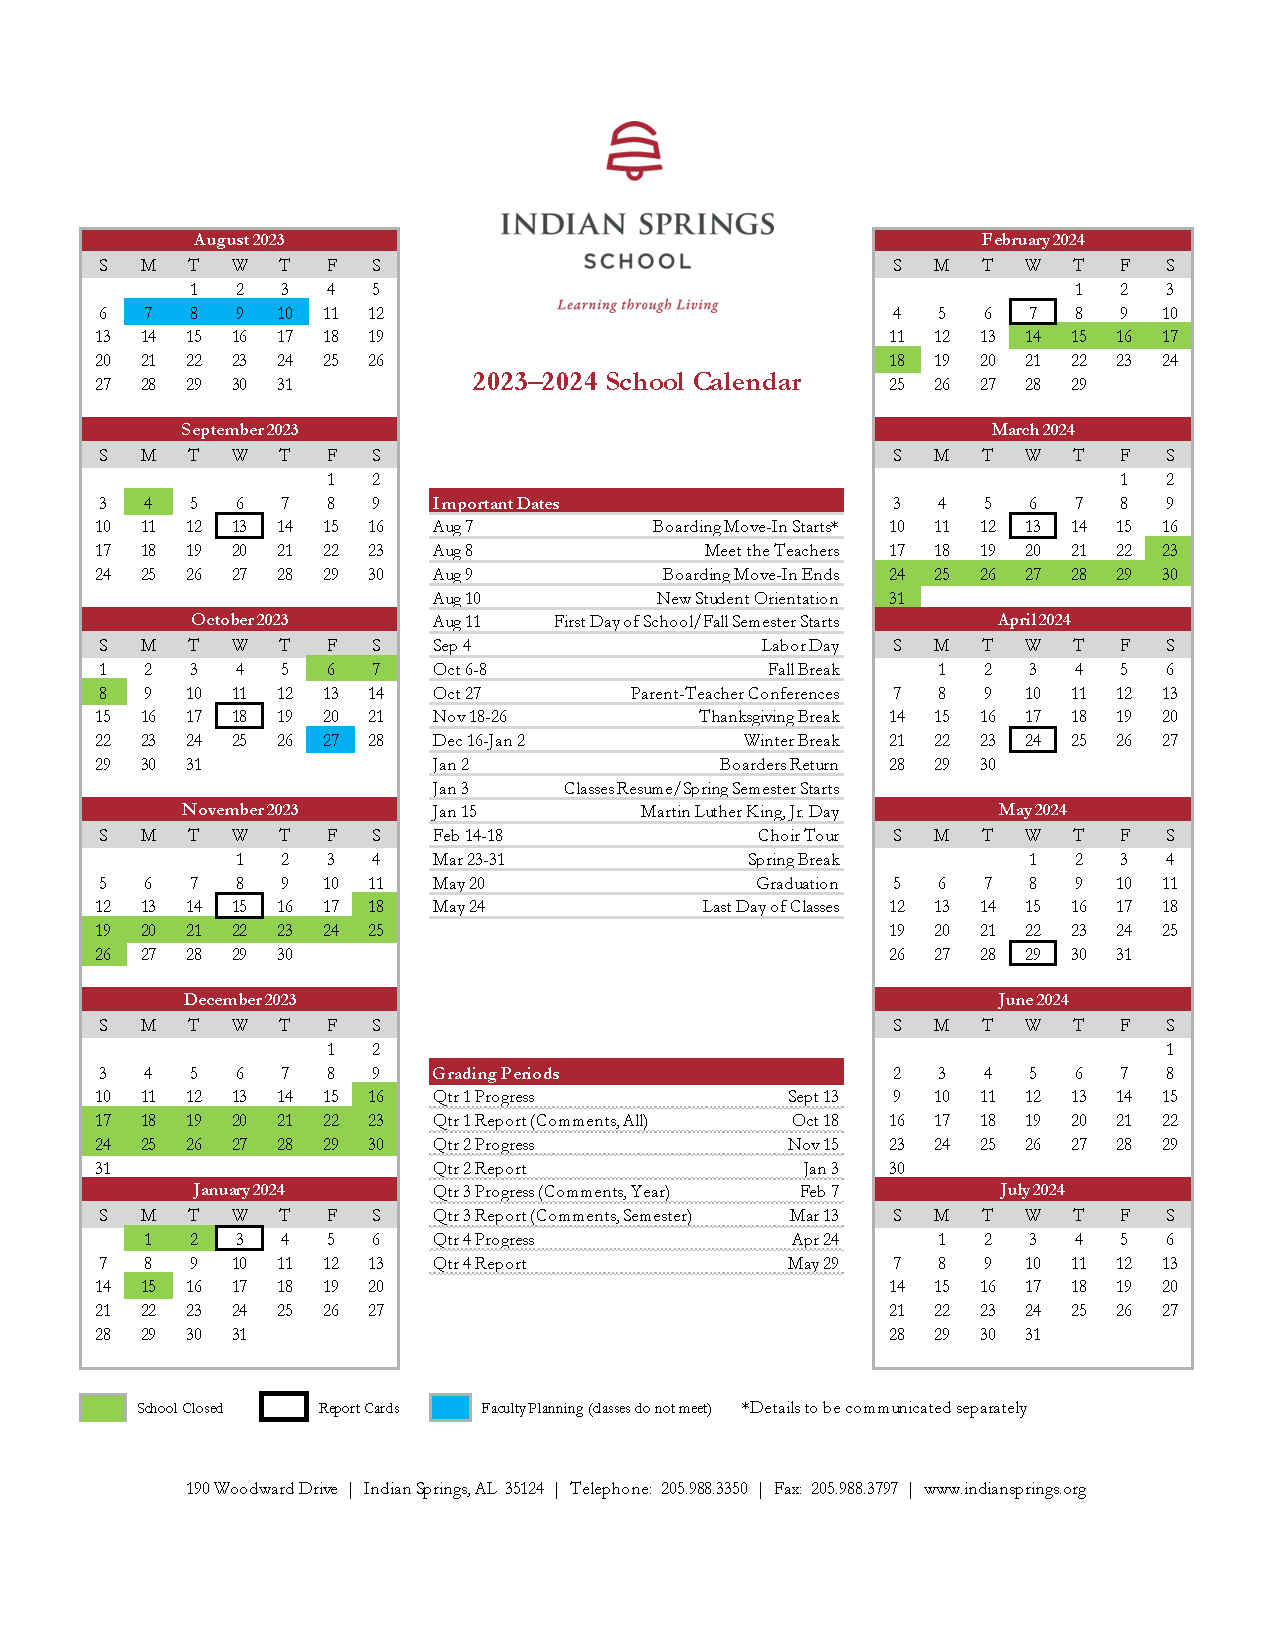
\includegraphics[scale=.9]{onepage2324.pdf}


